\chapter{Analyse der Datenstrukturen und Ableitung eines Trainingsformats}
\label{chap:analyse_der_datenstrukturen}

\section{Analyse der Ausgangsdaten}

Die Datengrundlage für das entwickelte System bilden EPLAN-Artikel \parencite{EPLANArtikelverwaltung} und EPLAN-Fenstermakros \parencite{EPLAN-Makros}. Diese liegen in Form von strukturierten XML-Dateien und .ema-Dateien, einem XML-ähnlichen Format, vor \parencite{srcStep911}.
Um diese Daten für ein Learning-to-Rank-System nutzbar zu machen, müssen diese zunächst aufbereitet und in ein maschinenverständliches Format überführt werden.

Das Ziel der Datenaufbereitung besteht darin, alle technisch wichtigen Informationen der EPLAN-Artikel \parencite{EPLANArtikelverwaltung} sowie die strukturellen Merkmale der EPLAN-Fenstermakros \parencite{EPLAN-Makros} zu extrahieren. Auf dieser Grundlage kann die Eignung eines EPLAN-Artikels \parencite{EPLANArtikelverwaltung} für ein EPLAN-Fenstermakro \parencite{EPLAN-Makros} bewertet werden. 
Die Umsetzung dieser Datenaufbereitung erfolgt innerhalb der entwickelten Trainings- und Rankingpipeline \parencite{srcStep911,srcPipeline}.

\section{Analyse der Makrostrukturen}

Die Analyse der Makrostrukturen der EPLAN-Fenstermakros \parencite{EPLAN-Makros} konzentriert sich auf die enthaltenen Funktions- und Strukturmerkmale, welche die Grundstruktur und Funktionalität der Makros bestimmen \parencite{srcStep911}.
Tabelle \ref{tab:makrostrukturmerkmale} fasst die analysierten Merkmalsgruppen, die jeweils extrahierten Informationen und deren Bedeutung zusammen.

\begin{table}[tbp]
    \centering
    \setlength{\tabcolsep}{4pt}
    \renewcommand{\arraystretch}{1.08}
    \caption{Analysierte Merkmalsgruppen der EPLAN-Fenstermakros}
    \label{tab:makrostrukturmerkmale}
    \begin{tabularx}{\textwidth}{>{\raggedright\arraybackslash}p{4.0cm} >{\raggedright\arraybackslash}X}
        \toprule
        \textbf{Merkmalsgruppe} & \textbf{Extrahierte Merkmale und Bedeutung} \\
        \midrule
        Function-Template-\newline Struktur &
        \textbf{Merkmale:} Function-Template-Kategorien, Function-Template-Gruppen, Function-Template-IDs, Function-Template-Sequenzen, Struktur-Hashes, Sequenz-Hashes.\newline
        \textbf{Bedeutung:} Function-Templates sind grundlegende Bausteine, welche die Funktionalität und Logik der EPLAN-Fenstermakros \parencite{EPLAN-Makros} im EPLAN-System \parencite{eplan2026} bestimmen. Die Merkmale beschreiben die funktionale Struktur und ermöglichen die Identifikation ähnlicher oder identischer Makrostrukturen. \\
        \addlinespace
        Anschluss- und\newline Signalstruktur &
        \textbf{Merkmale:} Anzahl der Anschlüsse, Anschlussrollen, Anschlussarten, Signalanzahlen, Kanalzahlen, I/O-Schemata, Klemmeninformationen.\newline
        \textbf{Bedeutung:} Beschreibt die technische Funktion sowie die Anschlusslogik eines EPLAN-Fenstermakros \parencite{EPLAN-Makros}. \\
        \addlinespace
        Geräteeigenschaften &
        \textbf{Merkmale:} Bus-Systeme, Steckersysteme, Safety-Eigenschaften, LED-Eigenschaften, Leistungsmerkmale, Kommunikationsinformationen.\newline
        \textbf{Bedeutung:} Ordnet Makros technisch im Maschinen- und Anlagenbau-Kontext ein. \\
        \addlinespace
        Varianten-\newline informationen &
        \textbf{Merkmale:} Variantenkennungen, Baugruppeninformationen, Konfigurationsmerkmale, produktspezifische Strukturinformationen.\newline
        \textbf{Bedeutung:} Unterstützt die Auflösung fachlich ähnlicher Varianten, die sich nur durch einzelne technische Eigenschaften oder Konfigurationsmerkmale unterscheiden. \\
        \bottomrule
    \end{tabularx}
\end{table}

Die Makrostrukturmerkmale werden beim Aufbau der Makrokandidatenprofile gespeichert. In der regulären Query-Kandidat-Feature-Berechnung werden diese jedoch nicht direkt mit einer unbekannten Artikelanfrage verglichen, da deren Zielmakrostruktur zur Anfragezeit nicht verfügbar ist.

\section{Aufbereitung der Artikeldaten}

Neben den vorhandenen EPLAN-Fenstermakros \parencite{EPLAN-Makros} werden auch die EPLAN-Artikeldaten \parencite{EPLANArtikelverwaltung} aufbereitet und analysiert \parencite{srcStep911}.
Die verwendeten Merkmalsgruppen sind in Tabelle \ref{tab:artikelmerkmale} zusammengefasst.

\begin{table}[tbp]
    \centering
    \setlength{\tabcolsep}{4pt}
    \renewcommand{\arraystretch}{1.08}
    \caption{Aufbereitete Merkmalsgruppen der EPLAN-Artikeldaten}
    \label{tab:artikelmerkmale}
    \begin{tabularx}{\textwidth}{>{\raggedright\arraybackslash}p{4.8cm} >{\raggedright\arraybackslash}X}
        \toprule
        \textbf{Merkmalsgruppe} & \textbf{Merkmale} \\
        \midrule
        Identifikationsmerkmale & Hersteller, Produktfamilie, Produkttyp, Bestellnummer, Produktcodes \\
        Elektrische Eigenschaften & Spannungswerte, Stromwerte, Leistungswerte, Frequenzangaben \\
        Mechanische Eigenschaften & Abmessungen, Gewicht, Baugrößen, Gehäusemerkmale \\
        Technologische Eigenschaften & Schutzarten, Kommunikationsstandards, Anschlussinformationen, spezielle Gerätefunktionen \\
        \bottomrule
    \end{tabularx}
\end{table}

Vor der Extraktion der Merkmale werden die Ursprungsdaten normalisiert und in ein einheitliches Format überführt. 
Dabei werden Texte, Schreibvarianten sowie technische Einheiten per Regular Expressions (RegEx) aufbereitet \parencite{srcStep911}.

\section{Erstellung von Makrokandidatenprofilen}

Im nächsten Schritt wird für jedes bekannte EPLAN-Fenstermakro \parencite{EPLAN-Makros} ein Makrokandidatenprofil erstellt. Ein Makrokandidatenprofil fasst dabei die technischen Eigenschaften des jeweiligen Makros zusammen. Für Merkmals-Kategorien werden die häufigsten Ausprägungen gespeichert. Für numerische Merkmale werden statistische Werte wie Mittelwert, Median, Minimum, Maximum und Häufigkeiten berechnet. 
Die Berechnung dieser Kandidatenprofile erfolgt innerhalb der Trainingspipeline \parencite{srcStep931,srcStep640}.

\section{Transformation in ein Rankingproblem}

Die Zuordnung der EPLAN-Fenstermakros \parencite{EPLAN-Makros} wird nicht als Klassifikationsproblem, sondern als Ranking-Aufgabe betrachtet. Für jede Anfrage werden alle EPLAN-Fenstermakro-Kandidaten \parencite{EPLAN-Makros} betrachtet, deren Profile ausschließlich aus dem Trainingssplit abgeleitet wurden. Eine vorgeschaltete Reduktion auf eine Top-$N$-Kandidatenmenge findet im aktuellen System nicht statt, sodass alle Trainingsartikel für die Paar-Bildung verwendet werden.

\begin{align}
    C_q = \{c_1,c_2,\dots,c_n\}
\end{align}

Dabei bezeichnet $q$ die Anfrage bzw. den Eingangsartikel, $C_q$ die Menge aller Makrokandidaten und $c_i$ einen einzelnen Makrokandidaten. Für jede Anfrage wird anschließend jeweils ein Paar $(q,c_i)$ gebildet. Dadurch entsteht eine Rankingstruktur, in der die Makrokandidaten gegeneinander bewertet werden.

\section{Berechnung der Pairwise-Merkmale}

Für jedes Paar von Anfrage und EPLAN-Fenstermakro-Kandidat \parencite{EPLAN-Makros} wird ein numerischer Feature-Vektor erzeugt. Die Merkmale der Paare lassen sich in mehrere Gruppen unterteilen: mengenbasierte Ähnlichkeiten, numerische Distanzmerkmale, Struktur- und Identitätsmerkmale sowie Retrieval-Merkmale.

Zur Bewertung von Merkmalsüberschneidungen wird unter anderem die Jaccard-Ähnlichkeit verwendet:

\begin{align}
    J(A,B) = \frac{|A \cap B|} {|A \cup B|}
\end{align}

Dabei bezeichnet $A$ die Merkmalsmenge der Anfrage und $B$ die Merkmalsmenge des Makrokandidaten. Der Wertebereich liegt zwischen 0 und 1.

Um numerische Eigenschaften zu bewerten, werden Differenzmerkmale berechnet. Die absolute Differenz ist definiert als:

\begin{align}
    d(x,y) = |x-y|
\end{align}

Die relative Differenz wird berechnet durch:

\begin{align}
    d_{rel}(x,y) = \frac{|x-y|} {\max(|x|,|y|,\varepsilon)}
\end{align}

Dabei bezeichnen $x$ den Eigenschaftswert der Anfrage, $y$ den Eigenschaftswert des Kandidaten und $\varepsilon$ eine kleine Konstante zur Vermeidung von Division durch Null. Durch diese Metriken können technische Kennwerte aus unterschiedlichen Größenordnungen verglichen werden.

Die weiteren Pairwise-Merkmale sind in Tabelle \ref{tab:pairwise_merkmale} zusammengefasst. BM25, Exact Match und Reciprocal Rank Fusion dienen im aktuellen System nicht als harte Kandidatenselektion. Sie werden für alle Makrokandidaten berechnet und als zusätzliche Merkmale an das Learning-to-Rank-Modell übergeben. Die theoretischen Grundlagen dieser Verfahren wurden bereits in Kapitel \ref{chap:stand_der_technik} erläutert. 
Die Berechnung der Pairwise-Merkmale erfolgt innerhalb der entwickelten Trainingspipeline \parencite{srcStep931,srcStep640}.

\begin{table}[tbp]
    \centering
    \setlength{\tabcolsep}{4pt}
    \renewcommand{\arraystretch}{1.08}
    \caption{Gruppen der Pairwise-Merkmale}
    \label{tab:pairwise_merkmale}
    \begin{tabularx}{\textwidth}{>{\raggedright\arraybackslash}p{3.6cm} >{\raggedright\arraybackslash}X}
        \toprule
        \textbf{Merkmalsgruppe} & \textbf{Merkmale und Funktion im Ranking} \\
        \midrule
        Mengenbasierte Ähnlichkeiten & \textbf{Merkmale:} Jaccard-Ähnlichkeit und Merkmalsüberschneidungen.\newline \textbf{Funktion:} Bewertung gemeinsamer technischer Eigenschaften von Anfrage und Kandidat \\
        \addlinespace
        Numerische Distanzmerkmale & \textbf{Merkmale:} Absolute und relative Differenzen technischer Kennwerte.\newline \textbf{Funktion:} Vergleich von Größenordnungen, Einheiten und technischen Wertebereichen \\
        \addlinespace
        Struktur- und Identitätsmerkmale & \textbf{Merkmale:} Produktcode-Matches, Strukturhash-Übereinstimmungen, Function-Template-Übereinstimmungen, Kanalzahlvergleiche, Variantenmerkmale, I/O-Strukturvergleiche.\newline \textbf{Funktion:} Beschreibung der technischen Identität eines Kandidaten \\
        \addlinespace
        Retrieval-Merkmale & \textbf{Merkmale:} BM25-Scores, Exact-Match-Scores, RRF-Scores, Retrieval-Ränge.\newline \textbf{Funktion:} Zusätzliche Trainingssignale für textuelle und exakte Übereinstimmungen \\
        \bottomrule
    \end{tabularx}
\end{table}

\section{Erzeugung der Relevanzlabels}

Für jedes Anfrage-Kandidaten-Paar wird ein Relevanzlabel erzeugt, das angibt, ob der Kandidat für die jeweilige Anfrage relevant ist oder nicht \parencite{srcStep931}.
Im verwendeten Trainingsmodus existiert pro Anfrage genau ein korrektes EPLAN-Fenstermakro \parencite{EPLAN-Makros}. Die Funktion für die Relevanz lautet:

\begin{align}
    y(q,c) = \begin{cases} 1, & \text{wenn } c \text{ das Zielmakro von } q \text{ ist} \\ 0, & \text{sonst} \end{cases}
\end{align}

Dabei bezeichnet $y(q,c)$ das Relevanzlabel, $q$ die Anfrage und $c$ den Makrokandidaten. Jede Anfragegruppe enthält genau einen positiven Kandidaten und mehrere negative Kandidaten. Die negativen Kandidaten sind dazu da, das Modell darauf zu trainieren, irrelevante Makros korrekt zu erkennen und von relevanten zu unterscheiden. 
Dadurch werden nicht einzelne Objekte klassifiziert, sondern die korrekte Sortierung der Menge an Kandidaten \parencite{srcStep931}.

\section{Erstellung des Trainingsformats}

Die berechneten Merkmale werden als Matrix gespeichert. Jede Zeile steht für ein Anfrage-Kandidat-Paar \parencite{srcStep931}:

\begin{align}
    (q,c_i) \rightarrow [x_1,x_2,\dots,x_n]
\end{align}

Dabei bezeichnet $q$ die Anfrage, $c_i$ den Makrokandidaten und $x_1,\dots,x_n$ die berechneten Features. Zusätzlich wird die Zuordnung jeder Anfrage zu einer Gruppe von Kandidaten gespeichert:

\begin{align}
    G_q = \{(q,c_1),(q,c_2),\dots,(q,c_n)\}
\end{align}

Dabei beschreibt $G_q$ die Menge aller Anfrage-Kandidat-Paare für die Anfrage $q$. Die Informationen aus den Gruppen werden zusammen mit den Featurevektoren an den LambdaRANK-Algorithmus übergeben \parencite{srcStep931}. 
Dadurch können die Kandidaten innerhalb derselben Anfrage gegeneinander bewertet werden und somit die optimale Rangfolge erlernt werden.

\section{Vermeidung von Zielinformations-Leakage}

Eine weitere wichtige Anforderung beim Aufbau der Trainingsdaten ist die Vermeidung von Zielinformations-Leakage. Dabei darf die Query-Seite ausschließlich Informationen enthalten, die aus eingehenden EPLAN-Artikeln \parencite{EPLANArtikelverwaltung} abgeleitet werden können. Informationen über das direkte Ziel-Fenster-Makro \parencite{EPLAN-Makros} dürfen nicht in die Eingabeseite einfließen.

Für die regulären Pairwise-Merkmale wird die Query-Seite auf Informationen beschränkt, die aus einem eingehenden Artikel abgeleitet werden können. Bezeichnungen wie \texttt{target\_macro} und \texttt{target\_family} sowie Strukturinformationen aus Makros werden für diese Query-Darstellung ausgeschlossen \parencite{srcLeakageGuard,srcStep640}.

Die Makrostrukturmerkmale werden dagegen in den Kandidatenprofilen gespeichert. Sie beschreiben somit zusätzlich die Eigenschaften eines zu bewertenden EPLAN-Fenster-Makros \parencite{EPLAN-Makros} und können für kandidatenbezogene Merkmale genutzt werden, ohne dass das Ziel-Fenster-Makro \parencite{EPLAN-Makros} direkt als Labelinformation in die Query eingeht \parencite{srcLeakageGuard}.

Eine genauere Betrachtung der Leakage-Sicherheit erfolgt im Kapitel \ref{chap:evaluierungskonzept_und_ergebnisse}.


Für eine bessere Veranschaulichung des Datenflusses innerhalb der Datenaufbereitung für das Training wird in Abbildung \ref{fig:trainingsformat_pipeline} ein schematisches Diagramm dargestellt.

\begin{figure}[tbp]
    \centering
    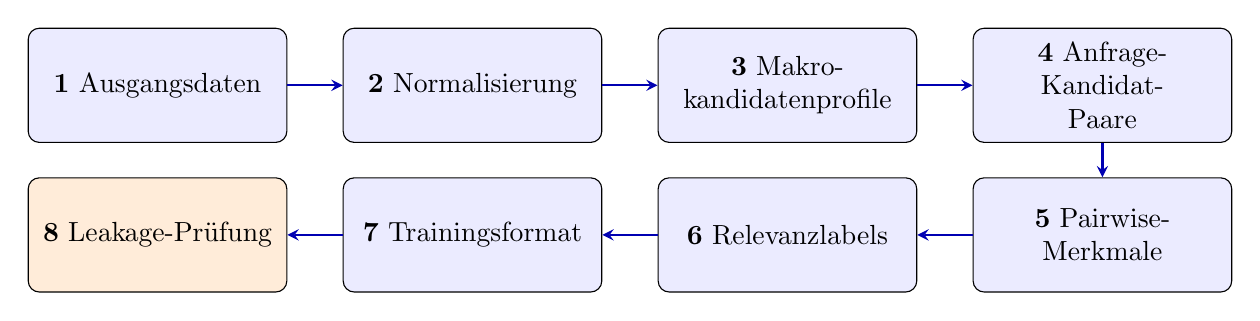
\begin{tikzpicture}[
        label distance=0.2cm,
        >=stealth,
        font=\normalsize,
        pipelinebox/.style={draw, rounded corners, fill=blue!8, text width=3.05cm, minimum height=1.45cm, inner ysep=0pt, align=center},
        check/.style={draw, rounded corners, fill=orange!15, text width=3.05cm, minimum height=1.45cm, inner ysep=0pt, align=center},
        flow/.style={->, thick, blue!70!black}
    ]
        \node[pipelinebox] (raw) at (0, 0) {\textbf{1} Ausgangsdaten};
        \node[pipelinebox] (norm) at (4.0, 0) {\textbf{2} Normalisierung};
        \node[pipelinebox] (profiles) at (8.0, 0) {\textbf{3} Makro-\\kandidatenprofile};
        \node[pipelinebox] (pairs) at (12.0, 0) {\textbf{4} Anfrage-Kandidat-\\Paare};

        \node[pipelinebox] (features) at (12.0, -1.9) {\textbf{5} Pairwise-\\Merkmale};
        \node[pipelinebox] (labels) at (8.0, -1.9) {\textbf{6} Relevanzlabels};
        \node[pipelinebox] (format) at (4.0, -1.9) {\textbf{7} Trainingsformat};
        \node[check] (leakage) at (0, -1.9) {\textbf{8} Leakage-Prüfung};

        \draw[flow] (raw) -- (norm);
        \draw[flow] (norm) -- (profiles);
        \draw[flow] (profiles) -- (pairs);
        \draw[flow] (pairs) -- (features);
        \draw[flow] (features) -- (labels);
        \draw[flow] (labels) -- (format);
        \draw[flow] (format) -- (leakage);
    \end{tikzpicture}
    \caption{Verarbeitungsschritte von den Ausgangsdaten bis zum Trainingsformat.}
    \label{fig:trainingsformat_pipeline}
\end{figure}
